\label{sec:intro}

With the development of algorithms and computation platforms, a single moving robot can navigate and build map in a novel environment. The cooperation of different robots can greatly improve the system capability, and the multi-robot system is a promising research field.

Distributed Simultaneously Localization and Mapping (DSLAM)~\cite{corah2019communication, cieslewski2018data}, which provides the status of different robots and the environment, is a fundamental problem for multi-robot systems, including multi-robot navigation \cite{tanner2005towards} and rescue \cite{baxter2007multi}. As illustrated in \Cref{fig:DSLAMframe}, there are three function thread on each robot, Visual Odometry (VO), Map Building (Map) and Place Recognition (PR). VO reads two time adjacent input images and calculates the relative pose between these images, and finial produces the trajectory of the robots. PR generates compact image representation to produce the candidate place recognition matches between different robots. Map thread records trajectory and builds the environment into local map.

\begin{figure*}[t]
    \begin{minipage}[t]{0.3\linewidth}  
    \centering
    \subfigure[ DSLAM framework. Each frame is fed to VO to calculate trajectory. The local map is build based on the trajectory. Some key frames are fed to PR to encode the scenes into descriptors for inter-robot scene matching. When the same scene is detected with different robots, the local maps of these robots are merged into global map. In this work, we adopt panoramic camera and CNN to DSLAM system. Use topology map for both PR and Map.
    ] {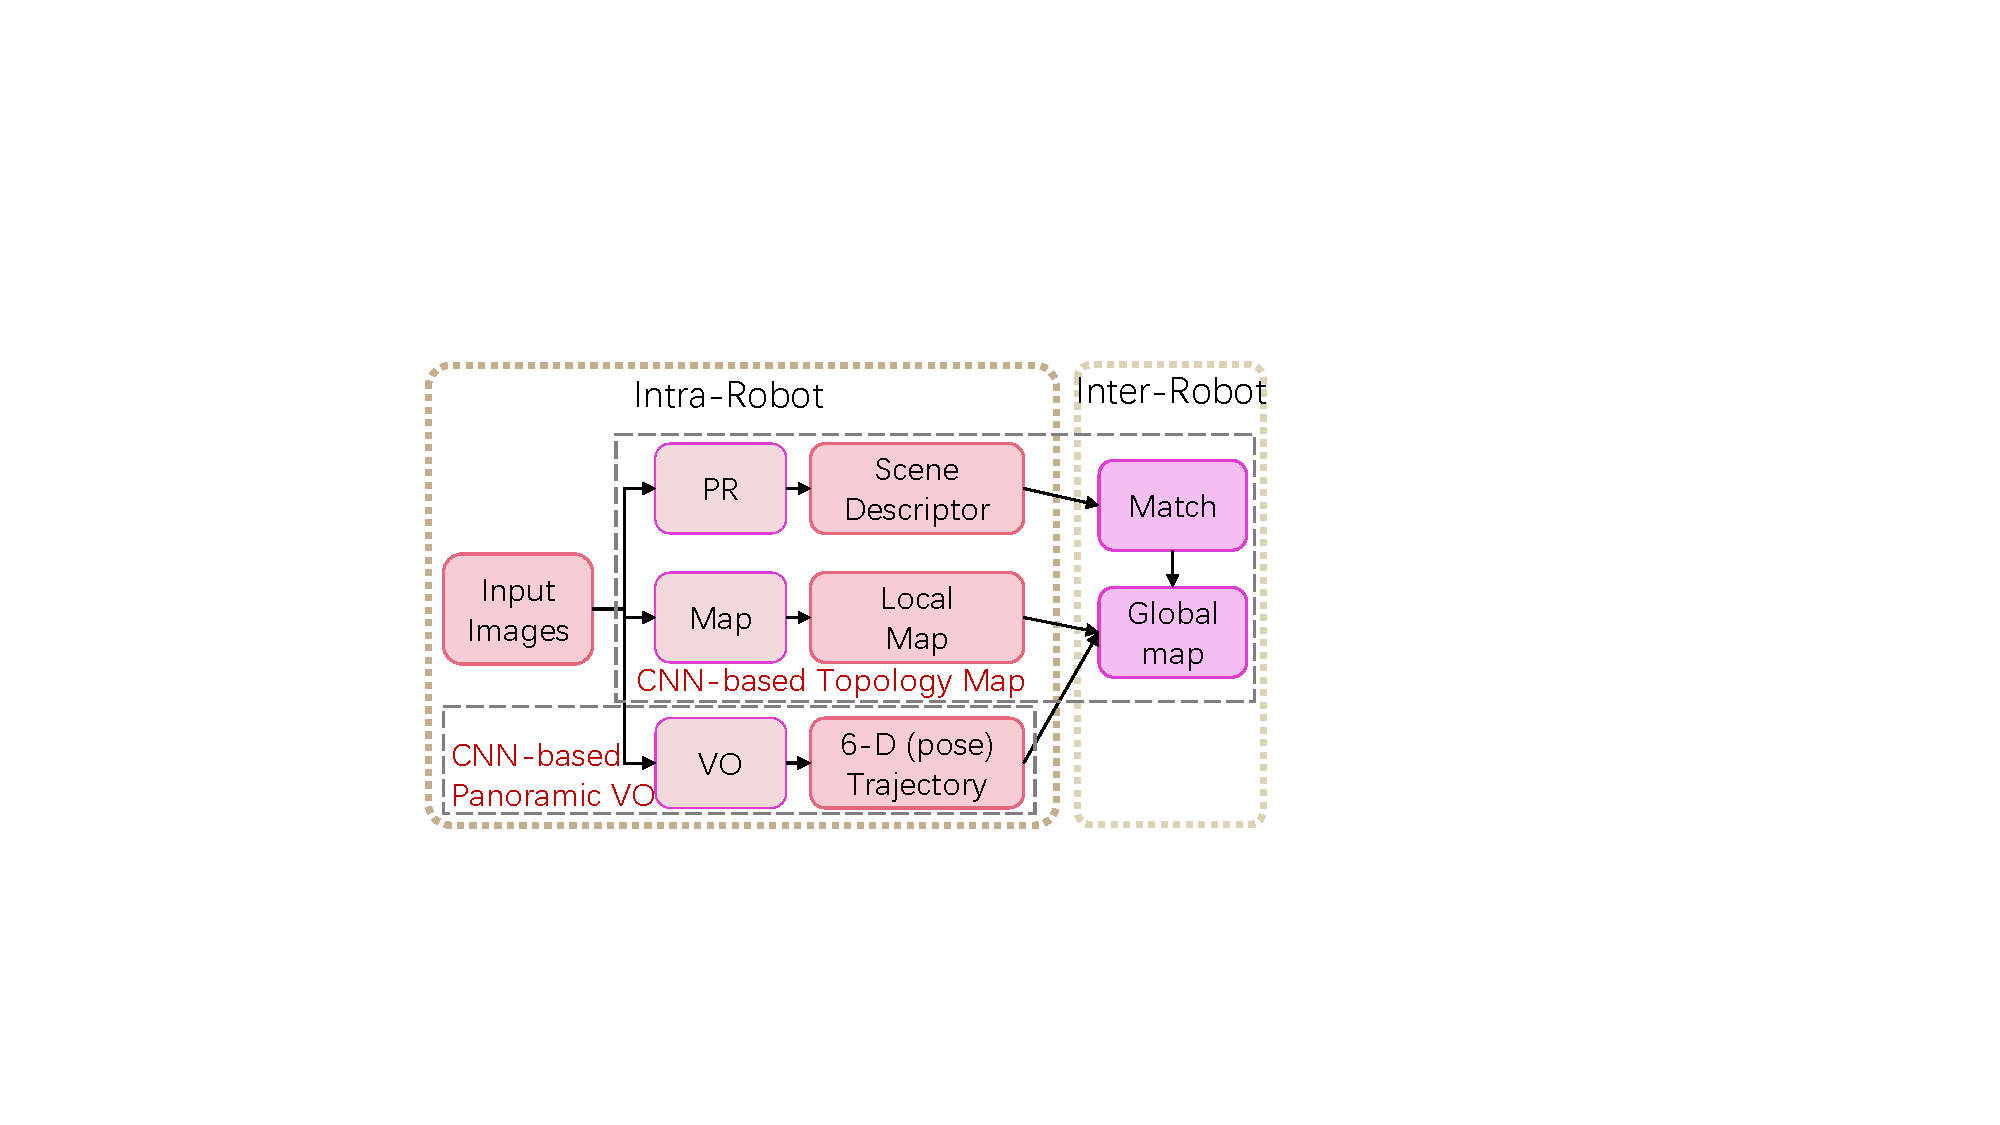
\includegraphics[width=0.95\textwidth]{fig/DSLAMframe.pdf}\label{fig:DSLAMframe}}
    \end{minipage}
    \begin{minipage}[t]{0.7\linewidth}  
    \centering  
    \subfigure[ Our CNN-based DSLAM system with panoramic camera. For VO, we use CNN to calculated the poses between different splited panoramic image frames \textcircled{1} and use graph optimization to fine-tune the camera pose of adjacent time. For Map and PR, we adopt CNN to generate descriptors \textcircled{3} for place recognition and build topology map based on the descriptors \textcircled{4}. We derectly match the topology map between robots \textcircled{5} and merge the local topology map \textcircled{6}.
    ] {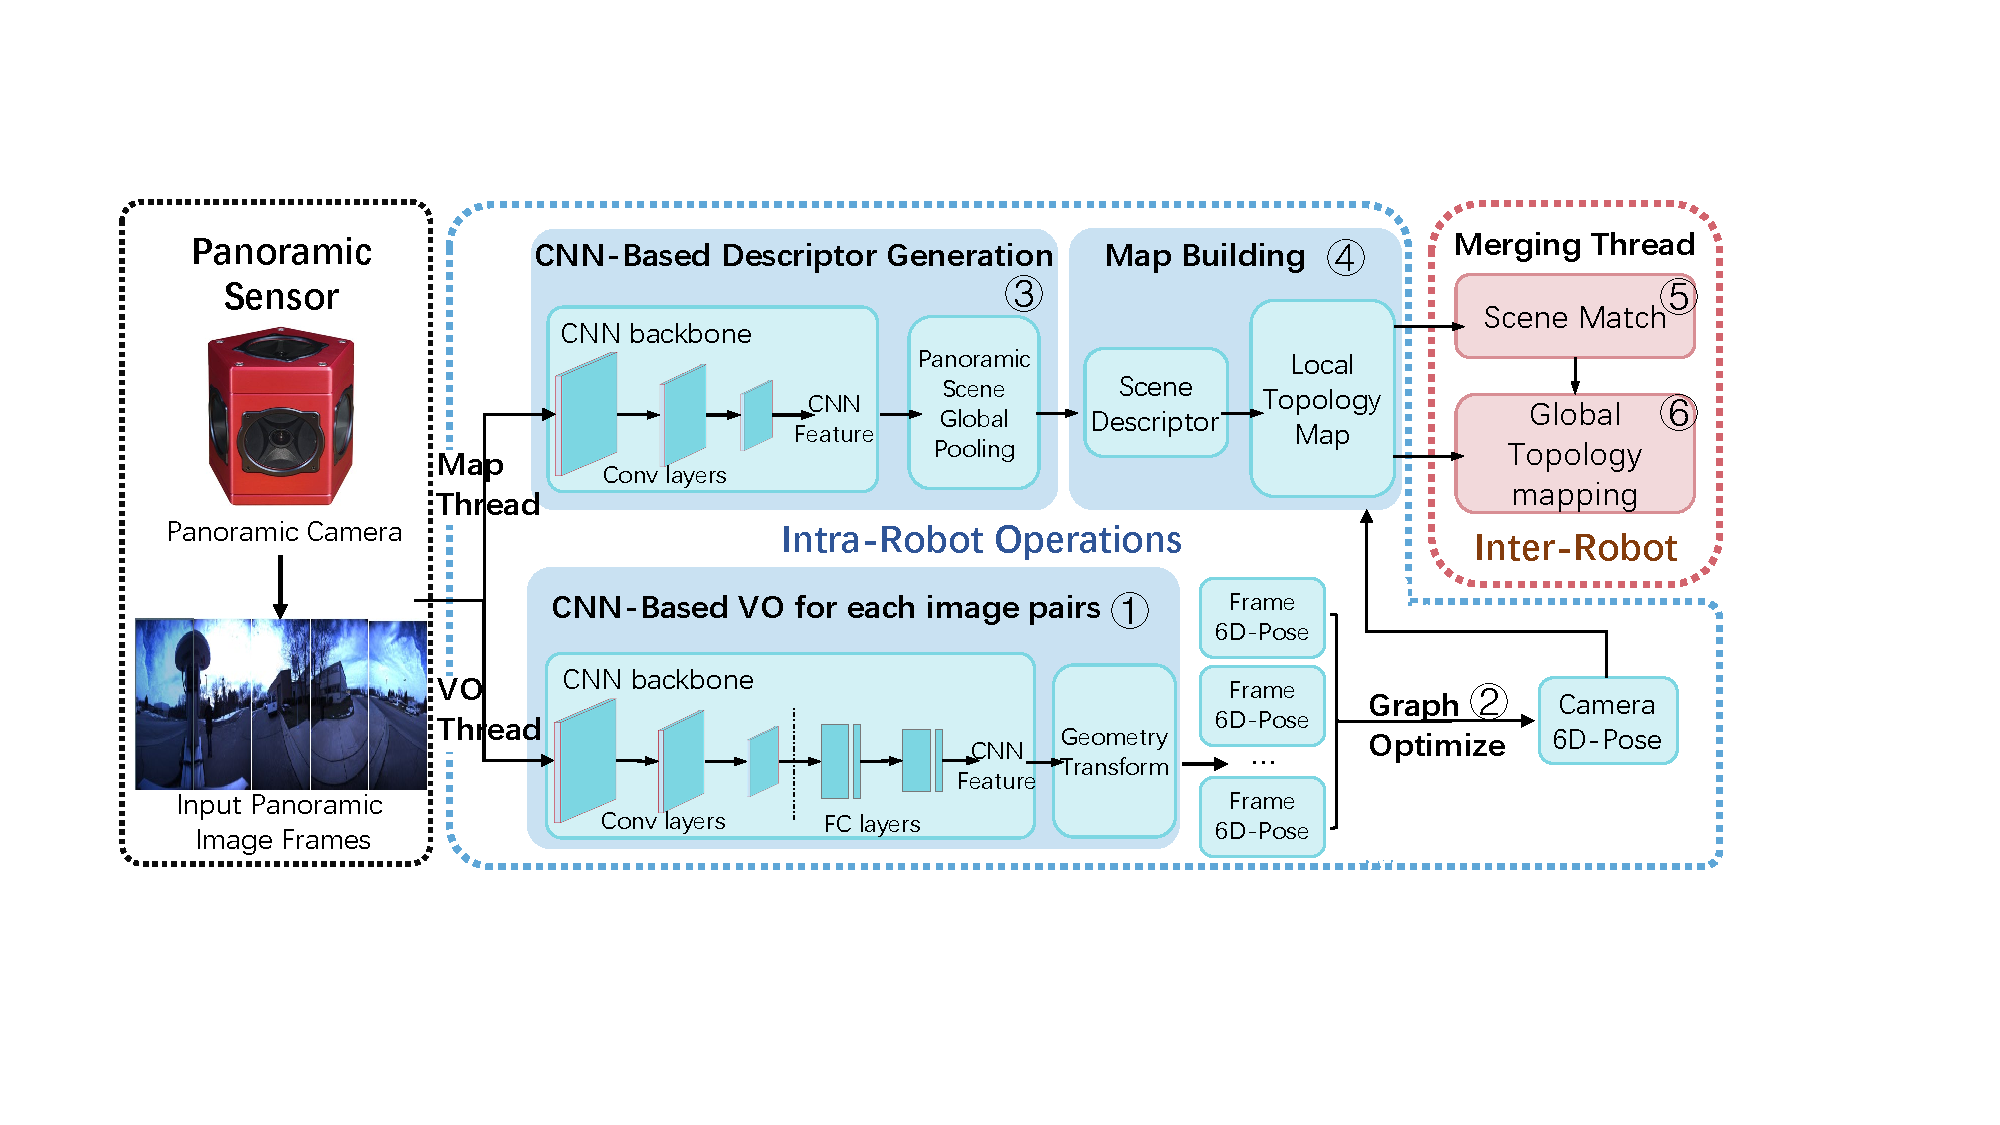
\includegraphics[width=0.95\linewidth]{fig/framework.pdf}\label{fig:framework}} 
    \end{minipage}
    \caption{DSLAM overview. \Cref{fig:DSLAMframe} shows the general DSLAM framework. \Cref{fig:framework} shows our CNN-based method with panoramic camera and topology map.
    }
\label{fig:overview}
\end{figure*}